Voor de eerste dataset, gegenereerd door $f(x,y)=sin((2x-1)^2+2y)$ op elk punt van het rooster toe te passen, worden de veeltermbenadering van graad $7$ in $x$ en $y$ in het interval $[-1,1]\times [-1,1]$ en de exacte functiewaarden weergeven op de linkse grafiek van figuur ~\ref{fig:oef12}. 
Voor de tweede dataset, gegenereerd door $F = \texttt{membrane}(1,15)$ in MATLAB, worden de veeltermbenadering van graad $7$ in $x$ en $y$ en de exacte data weergeven op de rechtse grafiek van figuur~\ref{fig:oef12}.

\begin{figure}[H]
    \centering
    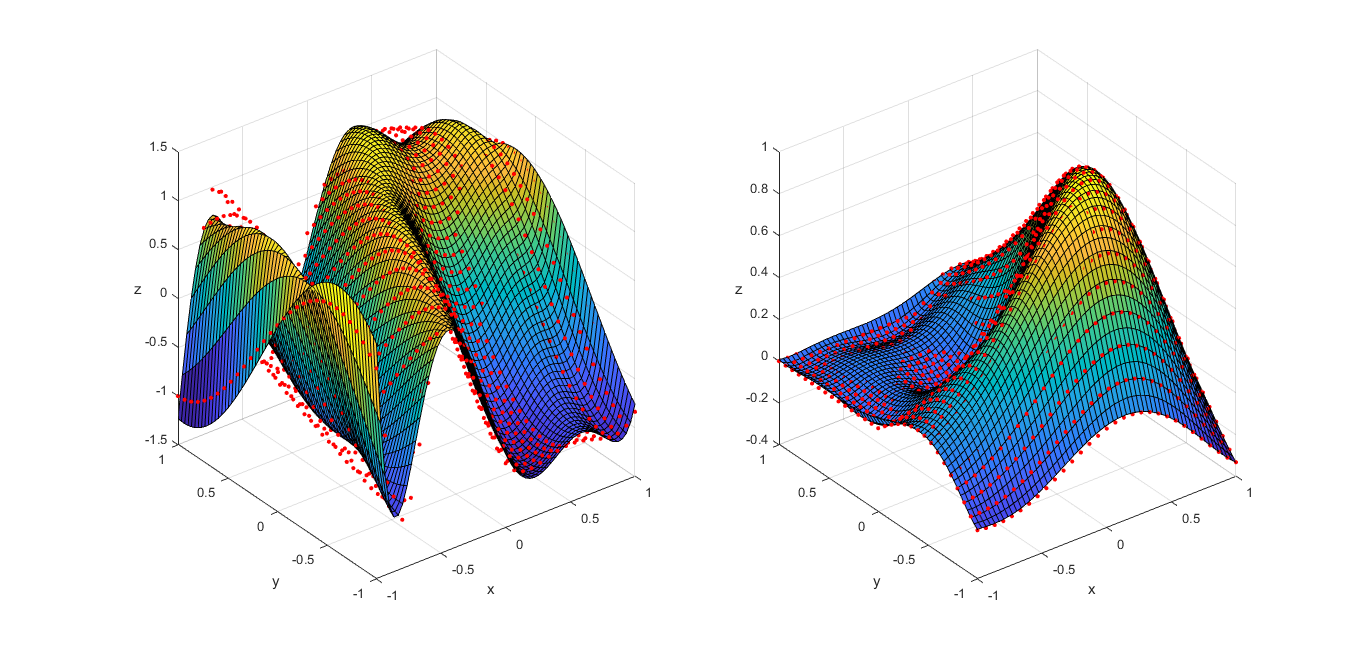
\includegraphics[width=1\textwidth]{oef12.png}
    \caption{veeltermbenadering van graad $7$ in $x$ en $y$ van de functie $f(x,y)=sin((2x-1)^2+2y)$ (links) en $F=\texttt{membrane}(1,15)$ (rechts)}
    \label{fig:oef12}
\end{figure}